\section{Methodology}
\label{sec:method}

We here describe the methodological approaches we designed for making ASCAs viable under noisy conditions. We initially present an overview of our methodology for handling noisy data in the proposed pipeline. Later, we discuss the required steps to implement our strategy. The steps are three. First, we describe how we built a SOTA baseline for the ASCAs task, benefiting from the long-range correlation capabilities of VTs. Second, we show how to apply LLMs to fix the spectrogram's ``typos'' with their interpretation abilities. Finally, we show how to fine-tune a model to bring it to the user's pockets.

\subsection{Threat Model}

This work considers two attack scenarios. First, \textbf{Phone Recording}, in which an attacker covertly places a smartphone or microphone-equipped device near a target’s keyboard to record keystroke sounds. Modern smartphone microphones effectively capture detailed acoustic signals from short distances. The attack assumes sensitive typing activity, such as passwords or confidential messages, occurring unnoticed by the victim. Such scenarios are realistic in public spaces, offices, or co-working environments where a hidden device can passively collect keystroke audio.

Second, \textbf{Zoom Recording}, executed remotely by capturing keystroke sounds transmitted through conferencing applications such as Zoom, MS Teams, or Google Meet. Unlike phone recordings, this method doesn't require physical proximity. Laptop microphones frequently transmit keystroke sounds despite built-in noise suppression, making residual acoustic information available. Given widespread remote work and virtual meetings, attackers monitoring audio streams can reconstruct sensitive inputs using machine learning. Studies indicate keystroke sounds persist even amid compression and bandwidth constraints, enhancing attack feasibility~\cite{compagno2017don}.

The adversary is assumed to have computational resources and expertise in deep learning-based ASCA methodologies. The attack involves capturing keystroke audio, generating Mel spectrograms, and classifying keystrokes using a transformer-based model (VTs) capable of modeling complex dependencies. To address potential errors due to noise, an LLM-based correction mechanism leverages contextual understanding to refine predictions, significantly improving keystroke recovery accuracy.

The success of these attacks depends on microphone sensitivity, typing speed, keyboard type, and environmental noise. Under controlled conditions, our VT-based classification achieves over 96\% accuracy, surpassing CNN-based techniques. In noisy conditions, integrating LLM-based error correction raises text recovery accuracy from approximately 50\% to over 90\%. These findings highlight vulnerabilities in keystroke-based systems and raise broader concerns for password authentication and digital communication security.


\subsection{Overview: Handling Noise}
\begin{figure*}[htbp]
    \centering
    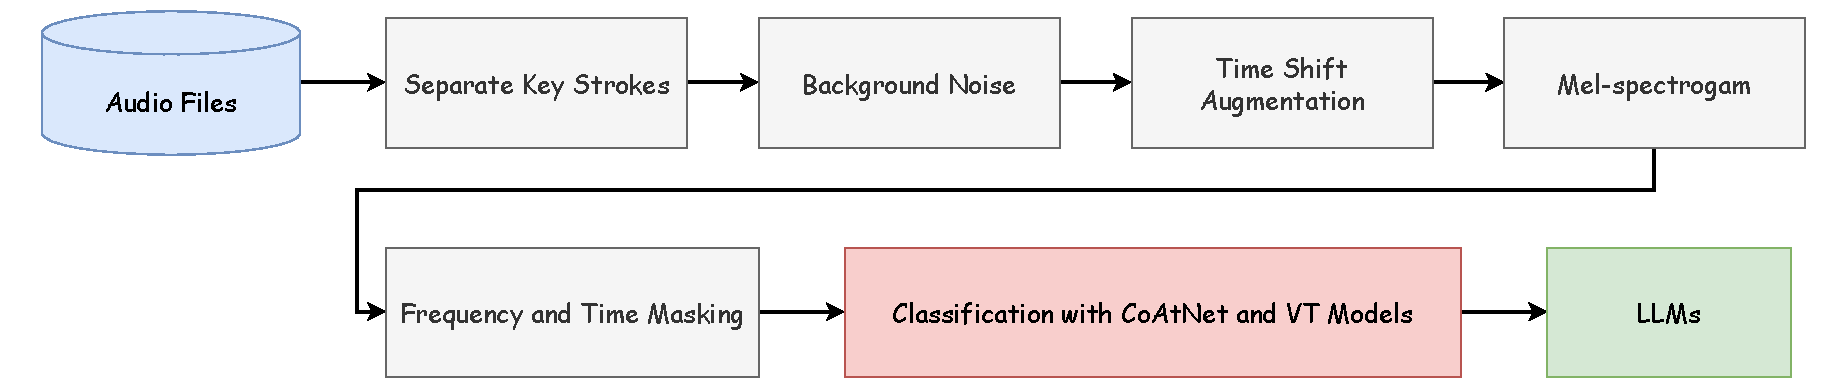
\includegraphics[width=\textwidth]{images/pipeline.pdf}
    \caption{Audio pre-processing pipeline for classification and LLM-based typo correction.}
    \label{fig:data_processing}
\end{figure*}

A key innovation in our design is the introduction of controlled noise in the audio signals, combined with additional random time-shifting of audio signals and random time and frequency masking applied to the mel-spectrogram representations. Specifically, we employ Gaussian noise at three levels—low, medium, and high—to analyze model robustness under challenging conditions. The noise is added directly to the waveform signal before the features are extracted. This makes sure that the degradation is realistic and sounds like background noise, such as chatter or hum.

The rationale behind introducing random time shifts is to account for the natural variations in keystroke timing that occur due to human typing inconsistencies and microphone delays. This step prevents models from overfitting to precise timing patterns, improving their generalization to real-world conditions. Similarly, the frequency and time masking that was used on the mel-spectrograms simulates the loss of information that can happen during real-life recordings, where spectral components may be partially blocked by the placement of the microphone or other sounds in the background.

In our experiments, noise augmentation was applied to the entire dataset—both during training and inference—to comprehensively evaluate model robustness. This ensures that the model encounters realistic noise conditions throughout the pipeline, rather than relying solely on clean training data.

Figure~\ref{fig:data_processing} provides an overview of the preprocessing pipeline. It shows how raw audio is turned into mel-spectrograms, which are then enhanced by steps such as adding noise, shifting time, and masking frequencies before classification. The figure also highlights the integration of LLMs for correcting noisy keystroke predictions, ensuring robust and contextually accurate outputs.

\subsection{Building a SOTA Baseline model}

Prior to addressing noise scenarios, we first developed a new SOTA model to be used as a baseline for performance measurements. Our concern is not to attribute to noise effects the impact actually caused by poor model performance. Therefore, we ensured to first build a reliable baseline that allowed us to isolate variables and further focus exclusively on noisy cases.

To build the new SOTA model, we utilized CoAtNet alongside five state-of-the-art vision transformer models: ViT~\cite{dosovitskiy2020image}, Swin~\cite{liu2021swin}, DeiT~\cite{touvron2021training}, CLIP~\cite{radford2021learning}, and BEiT~\cite{bao2021beit}. We selected CoAtNet for its hybrid architecture, combining convolutional and transformer-based processing. This architecture is ideal for mel-spectrogram classification, as it captures both local features and long-range dependencies.

Each additional VT model was included to ensure comprehensive evaluation, with each offering distinct advantages. ViT serves as a pure transformer-based benchmark, while Swin introduces efficient hierarchical feature extraction via shifted windows. DeiT is optimized for data efficiency, suited for limited-sample datasets. CLIP was tested for potential performance gains from its vision component, despite its multimodal nature. BEiT's masked image modeling pre-training allowed us to assess the benefits of strong visual pretraining in keystroke classification. This diverse selection enabled systematic evaluation and ensured our final choice was driven by empirical performance rather than arbitrary selection.

We used pre-trained VT models and fine-tuned them with our data. For the CoAtNet model, since the previous study's ~\cite{harrison2023practical} CoAtNet (it will be refered to it as B-CoAtNet for baseline CoAtNet) model does not specify the number of blocks or channel sizes, we configured the number of parameters to align with the smallest reported parameter size in the CoAtNet's original paper ~\cite{dai2021coatnet}. Notably, unlike the other selected VTs, CLIP is a multimodal model, meaning it incorporates both vision and language embeddings for downstream tasks. In our experiments, we exclusively utilized the vision component of the CLIP model, augmenting it with a fully connected layer before the softmax layer. 

\subsection{Finding and Fixing Errors with LLMs}
Detecting and correcting errors in noisy textual predictions is challenging due to the unpredictable nature of acoustic distortions. Unlike traditional spell-checking tasks, where errors follow common typing patterns, ASCA errors involve random character substitutions, deletions, or insertions caused by waveform perturbations. Thus, an LLM must infer missing or altered characters based on broader linguistic context, reconstructing meaningful sequences even without clear word boundaries (e.g., missing spaces). Our approach leverages few-shot prompting to adapt LLMs effectively to these distortions, ensuring robust correction across varying noise levels and keystroke misclassification patterns.

Detecting and correcting errors in noisy textual predictions is a critical step in enhancing the robustness of ASCA systems. This section details the methodology employed to address errors arising from noisy datasets by leveraging LLMs through few-shot prompting techniques. The process involves both datasets, noise environments, and evaluation metrics, providing a comprehensive analysis of error correction effectiveness. We did not consider a noise-free environment, as it is highly unlikely to encounter zero noise in real-world scenarios.

The selected sentences were mapped to acoustic data under different noise environments to simulate real-world scenarios, as shown in Table \ref{tab:noise_factors}. Noise factors were categorized as Low, Medium, and High. For each syllable or digit in a sentence, the corresponding sound wave was adjusted with noise using different noise factors. See Eq.~\ref{eq:add_noise} to see how noises are applied.
\begin{equation}
    S_{\text{noisy}} = S + \eta \cdot \mathcal{N}(0, 1)
\label{eq:add_noise}
\end{equation}
where $S$ indicates acoustic signal (i.e. sound wave) and $\eta$ is a noise factor.
We carefully selected noise factor values to ensure that the resulting accuracies for Low, Medium, and High noise levels were approximately 95\%, 85\%, and 70\%, respectively. The accuracy was calculated between the true sentence and sentence with errors. See Eq.~\ref{eq:accuracy} for more details. 
\par
\begin{equation}
    \text{Accuracy} = \frac{2 \cdot |M|}{|S_1| + |S_2|}
\label{eq:accuracy}
\end{equation}
\text{where:}
\begin{itemize}
    \item \( |M| \): The total number of matching characters between the two strings \( S_1 \) (the true sentence) and \( S_2 \) (the predicted sentence). Matches are determined by optimizing the alignment of characters, not restricted to contiguous sequences.
    \item \( |S_1| \): The length (number of characters) of the true sentence \( S_1 \).
    \item \( |S_2| \): The length (number of characters) of the predicted sentence \( S_2 \).
\end{itemize}
\begin{figure}[htbp]
    \centering
    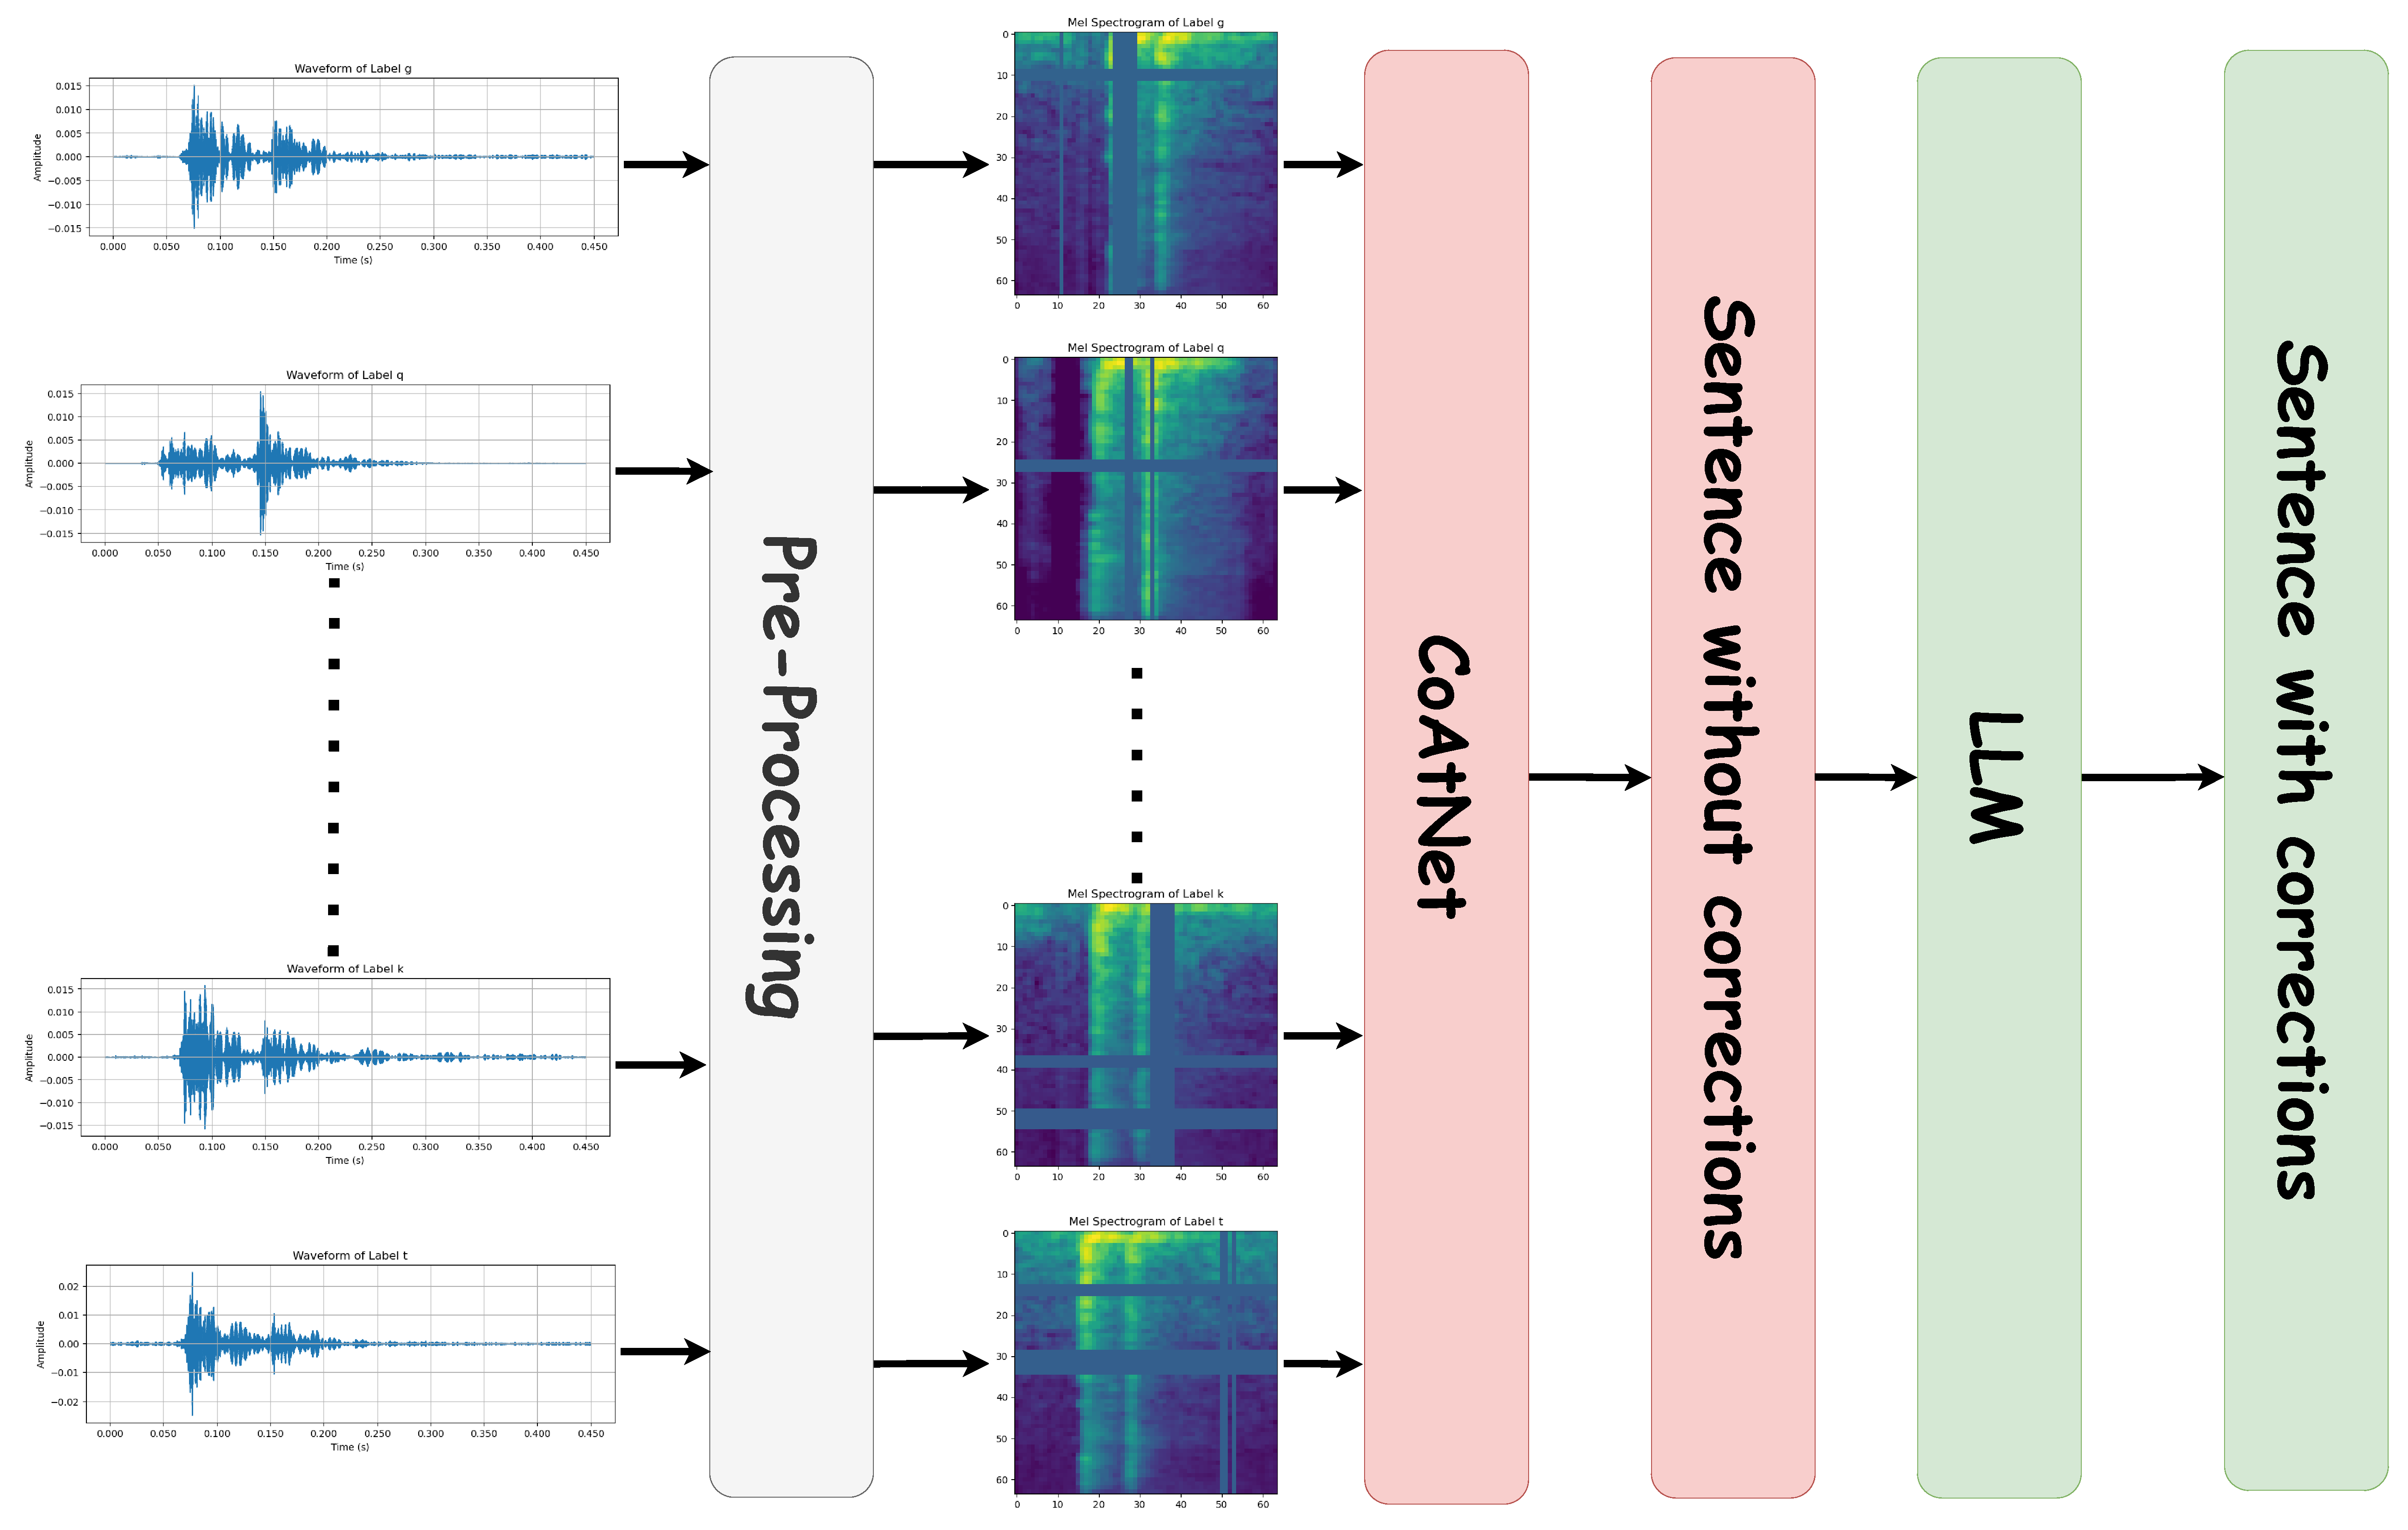
\includegraphics[width=\columnwidth]{images/figure_llm_pipeline.pdf}
    \caption{Pipeline for Detecting and Correcting Errors in Keystroke Predictions Using LLMs: From noisy audio waveforms to mel-spectrogram processing, keystroke classification via CoAtNet, and error detection/correction with LLMs, resulting in an accurate and more probable textual output.}
    \label{fig:pipeline}
\end{figure}
\par
The noisy audio waveforms were processed through the pipeline illustrated in Fig.~\ref{fig:pipeline}. After generating noisy textual predictions, typographical and semantic errors were corrected using LLMs. Few-shot prompting techniques, as outlined in Table~\ref{tab:prompt_structure}, were employed. The LLM was prompted with examples of sentences containing typos and their corrected counterparts. 
We utilized Llama-3.2-1B, Llama-3.2-3B, Llama-3.1-8B, and GPT-4o for LLM models.
The system prompt established the role of the LLM as an expert in correcting typos, while the user prompt included examples and the target sentence. 
\par 
\begin{table*}[htbp]
    \centering
    \begin{tabular}{p{1cm}|p{15cm}}
        \toprule
        \textbf{Role} & \textbf{Content} \\ \midrule
        \textit{System} & You are an expert in correcting typos in sentences. \\ 
        \midrule
        \textit{User} & Here are pairs of sentences with typos; learn from them: \\
             & \\
             & sentence: \{$S^{1}_{\text{pred}}$\} \\
             & corrected: \{$S^{1}_{\text{true}}$\} \\
             & \\
             & sentence: \{$S^{2}_{\text{pred}}$\} \\
             & corrected: \{$S^{2}_{\text{true}}$\} \\
             & \\
             & Now, please correct these sentences and output only the corrected version with no additional text: \{$S_{\text{pred}}$\} \\ 
        \bottomrule
    \end{tabular}
    \vspace{0.2em}
    \caption{Few-shot prompting structure for generating messages to correct typos using LLMs. The \textit{System} role sets the task context, and the \textit{User} role provides pairs of sentences (1) before correction $S_{\text{pred}}$ (sentence with errors) and (2) after correction $S_{\text{true}}$ (sentence without errors)}
    \label{tab:prompt_structure}
\end{table*}


\subsection{Detecting and Correcting Errors with Fine-tuned LLMs}
We hypothesized that GPT-4o could outperform smaller models (i.e., Llama family) in accurately correcting typos and mistakes in sentences. This is because models with a high number of parameters tend to perform better than smaller models. However, a significant drawback is its high inference time, attributed to its substantial model size ($\sim$200 billion parameters). To circumvent this issue, we propose a method to create a much smaller model specifically designed for typo correction task. We used Low-Rank Adaptation fine-tuning methods ~\cite{dettmers2023qloraefficientfinetuningquantized} to achieve the objective on the smaller model.
That is, instead of fine-tuning the full set of parameters in the model, a set of low-rank update matrices is introduced on top of the pre-trained weights to train the LLM for the error correction task. This allows task-specific learning without modifying the original weights, further reducing the computational cost and memory footprint.
\par
We took a pre-trained Llama-3.2-3B ($\sim$3 billion parameters) model and chose the more efficient QLoRA method ~\cite{unsloth} for the fine-tuning task. The smaller low-rank update matrices have a dimension of $d \times c$ where $d$ is the dimension of the original weight matrices, and $c$ is chosen arbitrarily but satisfying $d$ >{}> $c$.
%. The value of $d$ is much higher than 16 in general.
Training is carried out on specific training tasks where the predicted sentences from the audio are the input, and the correct output is the actual sentences being typed. To enhance the robustness of the model against noise, we progressively increase the noise level in the training data. Following Table \ref{tab:noise_factors}, the training for each dataset starts with a low noise factor and goes up to high noise intensity, one epoch for each noise level. AdamW optimizer, with a learning rate of 0.0002, is used for fine-tuning over three epochs: the first with low, the second with medium, and the third with high noise sentences.
% we show that this method of fine-tuning demonstrates great performance. This will be further discussed in the Results section.
% We prompt the model as described in Table \ref{tab:prompt_structure_ft}.
% This is different from the original prompting structure in Table \ref{tab:prompt_structure} 
Since we train the model on the error correction task specifically, zero-shot prompting is used. The gradient updates were only applied to the LoRA weights, while the original Llama weights were frozen. The updates can be expressed in Eq.~\ref{eq:lora_update}.
\begin{equation}
    W = W_0 + \Delta W = W_0 + AB
\label{eq:lora_update}
\end{equation}
where $W$ is the updated weight after fine-tuning, $W_0$ is the original pre-trained weight, and $\Delta W$ is the update being applied. Traditional fine-tuning directly operates on $\Delta W$, where $W, W_0, \Delta W \in \mathbb{R}^{d\times d}$ for large $d$. In contrast to traditional fine-tuning methods, we used QLoRA to operate on weighs $A, B$ where $A \in \mathbb{R}^{d\times c}, B \in \mathbb{R}^{c\times d}$ for a much smaller $c$. Instead of computing $\Delta W$ directly, we calculate $\Delta W = AB$ and only make updates on small matrices $A$ and $B$.
\par
Concluding the methodology section, our comprehensive approach demonstrates the robustness of the (fine-tuned) LLM-based error detection and correction framework across diverse noise environments and datasets. 
The results, presented in the subsequent section, demonstrate the performance improvements achieved by integrating LLMs with the ASCA pipeline, offering insights into their potential for real-world applications.
